\documentclass[12pt]{article}
\usepackage{graphicx} % Required for inserting images
\usepackage{amsmath}
\usepackage{placeins}

\begin{document}

\begin{titlepage}
    \begin{center}
        \huge
        Butterworth IIR\\Filter Design Report
        \vfill
        \large
        Student Details:\\\vspace{3pt}
        Name: Kanak Yadav\\\vspace{3pt}
        Roll No: 20D070044\\\vspace{3pt}
        Filter Number: 55\\\vspace{3pt}
        Group Number: 37\\\vspace{60pt}
        Reviewer Details:\\\vspace{3pt}
        Name: Pal Abhijeet Manoj\\\vspace{3pt}
        Roll No: 200100107
        \vfill
    \end{center}
\end{titlepage}

\section{Design}
\subsection{Un-normalized Discrete Time Filter}
The un-normalized discrete time filter specifications are uniquely assigned to each student using the filter number assigned to them.

The Butterworth filter to be designed is a bandpass filter for filter numbers 1 to 80 and a bandstop for filter numbers 81 to 160.

Hence, we would be designing a Butterworth IIR Bandpass Filter.

The passband for the bandpass filter is BL(m) kHz to BH(m) kHz, which are defined as:
\begin{align*}
    BL(m) &= 10 + 5 q(m) + 13 r(m),\\
    BH(m) &= BL(m) + 75,
\end{align*}
where,
\begin{align*}
    q(m) &= \text{greatest integer} < 0.1m, \text{and}\\
    r(m) &= m - 10q(m).
\end{align*}
For the assigned filter number m,
\begin{align*}
    q(m) &= \text{greatest integer} < 5.5\\
    &= 5,\\
    r(m) &= 55 - 10(5)\\
    &= 5.
\end{align*}
Substituting the values of q(m) and r(m), we get
\begin{align*}
    BL(m) &= 10 + 5(5) + 13(5)\\
    &= 100,\\
    BH(m) &= 100 + 75\\
    &= 175.
\end{align*}
Thus, the passband edges are:
\begin{align*}
    f_{p1} &= 100 kHz,\\
    f_{p2} &= 175 kHz.
\end{align*}
The transition bandwidth is given to be\[\Delta_f = 5 kHz.\]
Thus, the stopband edges are:
\begin{align*}
    f_{s1} &= f_{p1} - \Delta_f = 95 kHz,\\
    f_{s2} &= f_{p1} + \Delta_f = 180 kHz.
\end{align*}

Now we can state the specifications of the discrete-time bandpass filter.
\newline
\hline
\vspace{10pt}
\textbf{Specifications:}
\begin{itemize}
    \item Passband: 100 kHz to 175 kHz,
    \item Stopband: 0 to 95 kHz and 180 kHz to 300 kHz (since $f_s$ = 600 kHz),
    \item Passband and Stopband tolerance: 0.15,
    \item Passband and Stopband nature: Monotonic.
\end{itemize}
\hline

\subsection{Normalized Digital Filter}
Given that our signal of interest is bandlimited to
\[f_b = 280 kHz,\]
to satisfy the Nyquist Criterion,
\[f_s > 2 f_b = 560 kHz.\]
Given sampling frequency is
\[f_s = 600 kHz > 560 kHz.\]
Hence, the Nyquist criterion is satisfied.

For normalizing the frequencies, we need to make the sampling frequency map to $2\pi$. Thus,
\[\omega = \frac{2\pi f}{f_s}\]
\newpage
This gives us the normalized digital frequencies as follows:
\begin{table}[h]
    \centering
    \begin{tabular}{|c|c|}\hline
         Discrete time frequency&Normalized digital frequency\\
         $f$ (kHz)&$\omega$ (radians)\\\hline
         0&0\\\hline
         95&$\omega_{s1}$ = 0.9948377\\\hline
         100&$\omega_{p1}$ = 1.0471976\\\hline
         175&$\omega_{p2}$ = 1.8325957\\\hline
         180&$\omega_{s2}$ = 1.8849556\\\hline
         300&$\pi$\\\hline
    \end{tabular}
    \caption{Normalizing frequency.}
    \label{tab:1}
\end{table}

Now we can state the specifications of the digital bandpass filter.
\newline
\hline
\vspace{10pt}
\textbf{Specifications:}
\begin{itemize}
    \item Passband: 1.0471976 to 1.8325957,
    \item Stopband: 0 to 0.9948377 and 1.8849556 to  $\pi$,
    \item Passband and Stopband tolerance: 0.15,
    \item Passband and Stopband nature: Monotonic.
\end{itemize}
\hline

\subsection{Analog Bandpass Filter}
For converting the normalized digital specifications to the specifications for an analog filter of the same type (bandpass), we use the bilinear transformation:
\[s = \frac{1-z^{-1}}{1+z^{-1}},\]
substituting the values of s and z, we get
\begin{align*}
    j\Omega &= \frac{1-e^{-j\omega}}{1+e^{-j\omega}} = \frac{e^{j\omega/2}-e^{-j\omega/2}}{e^{+j\omega/2}+e^{-j\omega/2}}\\
    &= \frac{2j\sin(\omega/2)}{2\cos(\omega/2)} = j\tan(\omega/2)\\
    \Omega &= \tan(\omega/2)
\end{align*}
\newpage
This gives us the analog bandpass frequencies as:
\begin{table}[h]
    \centering
    \begin{tabular}{|c|c|}\hline
         Normalized digital frequency&Analog frequency\\
         $\omega$ (radians)&$\Omega$\\\hline
         0&0\\\hline
         0.9948377&$\Omega_{s1}$ = 0.5429557\\\hline
         1.0471976&$\Omega_{p1}$ = 0.5773503\\\hline
         1.8325957&$\Omega_{p2}$ = 1.3032254\\\hline
         1.8849556&$\Omega_{s2}$ = 1.3763819\\\hline
         $\pi$&$\infty$\\\hline
    \end{tabular}
    \caption{Applying the bilinear transformation.}
    \label{tab:2}
\end{table}

Now we can state the specifications of the digital bandpass filter.
\newline
\hline
\vspace{10pt}
\textbf{Specifications:}
\begin{itemize}
    \item Passband: 0.5773503 to 1.3032254,
    \item Stopband: 0 to 0.5429557 and 1.3763819 to  $\infty$,
    \item Passband and Stopband tolerance: 0.15,
    \item Passband and Stopband nature: Monotonic.
\end{itemize}
\hline

\subsection{Frequency Transformation}
We need to employ a frequency transformation to convert our bandpass filter specifications into those of a lowpass filter. For this, we use the frequency transformation derived from the impedance of a series LC circuit:
\[s_L = \frac{s^2 + \Omega_0^2}{Bs},\]
where the subscript L stands for Lowpass. $\Omega_0$ is the resonant frequency and B is the bandwidth of the series LC circuit. Substituting the values of s$_L$ and s, we get
\begin{align*}
    j\Omega_L &= \frac{(j\Omega)^2 + \Omega_0^2}{B(j\Omega)} = \frac{1}{j}\frac{(-\Omega^2 + \Omega_0^2)}{B\Omega}\\
    &= -j\frac{(-\Omega^2 + \Omega_0^2)}{B\Omega} = j\frac{(\Omega^2 - \Omega_0^2)}{B\Omega}\\
    \Omega_L &= \frac{\Omega^2 - \Omega_0^2}{B\Omega}
\end{align*}
Now, we have two degrees of freedom, $\Omega_0$ and B. We also decide to follow the convention that the passband edge of the lowpass filter, in both the positive and negative half of the $\Omega_L$ axis, has a magnitude of one. In other words, we want $\Omega_{p1}$ and $\Omega_{p2}$ to map to -1 and +1 respectively on the $\Omega_L$ axis. To achieve this, we solve the following two equations
\[-1 = \frac{\Omega_{p1}^2 - \Omega_0^2}{B\Omega_{p1}}\]
and
\[+1 = \frac{\Omega_{p2}^2 - \Omega_0^2}{B\Omega_{p2}}\]
By equating $\Omega_0^2$ we get
\begin{align*}
    \Omega_{p1}^2 + B\Omega_{p1} &= \Omega_{p2}^2 - B\Omega_{p2}\\
    B(\Omega_{p2} + \Omega_{p1}) &= \Omega_{p2}^2 - \Omega_{p1}^2\\
    B &= \Omega_{p2} - \Omega_{p1}
\end{align*}
Substituting the value of B, we get
\begin{align*}
    \Omega_0^2 &= \Omega_{p1}^2 + (\Omega_{p2} - \Omega_{p1})\Omega_{p1}\\
    \Omega_0^2 &= \Omega_{p1}^2 + \Omega_{p2}\Omega_{p1} - \Omega_{p1}^2 = \Omega_{p2}\Omega_{p1}\\
    \Omega_0 &= \sqrt{\Omega_{p2}\Omega_{p1}}
\end{align*}
By substituting the value of $\Omega_{p1}$ and $\Omega_{p2}$, we get
\begin{align*}
    B &= 1.3032254 - 0.5773503 = 0.7258751\\
    \Omega_0 &= \sqrt{(1.3032254)(0.5773503)} = \sqrt{0.7524175} \approx 0.8674200
\end{align*}
\newpage
\hline
\vspace{10pt}
\textbf{Transformation and Parameters}
\begin{itemize}
    \item Transformation:\[\Omega_L = \frac{\Omega^2 - \Omega_0^2}{B\Omega}\]
    \item Parameters:
    \begin{itemize}
        \item $\Omega_0$ = 0.8674200,
        \item B = 0.7258751
    \end{itemize}
\end{itemize}
\hline

\subsection{Analog Lowpass Filter}
Substituting the values of $\Omega_o$ and B, we get the frequency transformation to be employed as:
\[\Omega_L = \frac{\Omega^2 - (0.7524175)}{(0.7258751)\Omega}\]
This gives us the analog lowpass frequencies as:
\begin{table}[h]
    \centering
    \begin{tabular}{|c|c|}\hline
         Analog frequency&Analog Lowpass Frequency\\
         $\Omega$ &$\Omega_L$\\\hline
         0$^+$&$-\infty$\\\hline
         0.5429557&$\Omega_{Ls1}$ = -1.1611157\\\hline
         0.5773503&$\Omega_{Lp1}$ = -1\\\hline
         1.3032254&$\Omega_{Lp2}$ = 1\\\hline
         1.3763819&$\Omega_{Ls2}$ = 1.1430597\\\hline
         $\infty$&$\infty$\\\hline
    \end{tabular}
    \caption{Analog frequency transformation.}
    \label{tab:3}
\end{table}

The passband edge of the lowpass filter was specified to be one while employing the frequency transformation but, the stopband edge now has two possible values of which, we choose the more stringent value (the value with a smaller magnitude) since satisfying the stronger specifications will automatically satisfy the weaker specifications. Thus
\begin{align*}
    \Omega_p &= 1\\
    \Omega_s &= min(abs(\Omega_{Ls1}), abs(\Omega_{Ls1}))\\
    &= min(1.1611157, 1.1430597)\\
    \Omega_s &= 1.1430597
\end{align*}

Now we can state the specifications of the analog lowpass filter.
\newline
\hline
\vspace{10pt}
\textbf{Specifications:}
\begin{itemize}
    \item Passband: 0 to 1,
    \item Stopband: 1.1430597 to  $\infty$,
    \item Passband and Stopband tolerance: 0.15,
    \item Passband and Stopband nature: Monotonic.
\end{itemize}
\hline

\subsection{Butterworth Analog Lowpass Transfer Function}
The Butterworth analog lowpass transfer function is given as:
\[\text{H}_{\text{analog, LPF}}\text{(s}_\text{L}\text{)} = \frac{\Omega_c^N}{\prod_{k\epsilon LHP}(s - s_k)}.\]
$\Omega_c$ and N are given by the specifications as:
\[N \geq \frac{\log{\frac{D_2}{D_1}}}{2\log{\frac{\Omega_s}{\Omega_p}}},\]
\[\frac{\Omega_p}{D_1^\frac{1}{2N}} \leq \Omega_c \leq \frac{\Omega_s}{D_2^\frac{1}{2N}},\]
where $D_1$ and $D_2$ are given by:
\begin{align*}
    D_1 &= \frac{1}{(1 - \delta_1)^2} - 1,\\
    D_2 &= \frac{1}{\delta_2^2} - 1.
\end{align*}
$\delta_1$ and $\delta_2$ are the passband and stopband tolerances.
\begin{align*}
    D_1 &= \frac{1}{(1 - 0.15)^2} - 1 = 0.3840830\\
    D_2 &= \frac{1}{0.15^2} - 1 = 43.444444
\end{align*}
This gives us
\[N \geq \frac{\log(113.11211)}{2\log(1.1430597)} \approx 17.681654,\]
Hence, we choose\[N = 18.\]
Now,
\[\frac{1}{0.3840830^\frac{1}{2(18)}} \leq \Omega_c \leq \frac{1.143059}{43.444444^\frac{1}{2(18)}},\]
\[1.0269369 \leq \Omega_c \leq 1.0293682\]
We can choose any value for $\Omega_c$, so let's choose it to be the average of the two bounds.
\[\Omega_c = 1.0281525\]
Now the poles can be found by setting the denominator of the magnitude squared form of the Butterworth lowpass filter transfer function to zero.
\[|\text{H}_{\text{analog, LPF}}\text{(s}_\text{L}\text{)}|^2 = \frac{1}{1 + (\frac{s}{j\Omega_c})^{2N}}\]
\[1 + (\frac{s_k}{j\Omega_c})^{2N} = 0\]
\[(\frac{s_k}{j\Omega_c})^{2N} = -1 = e^{j(2k+1)\pi}\]
\begin{align*}
    \frac{s_k}{j\Omega_c} &= e^{j\frac{2k+1}{2N}\pi}\\
    s_k &= j\Omega_ce^{j\frac{2k+1}{2N}\pi}\\
    s_k &= \Omega_ce^{j(\frac{k\pi}{N}+\frac{\pi}{2N}+\frac{\pi}{2})}
\end{align*}
To obtain the LHP (Left Half Plane) poles, we need to take the values of k ranging from 0 to N-1.

Now we can find the Butterworth analog lowpass filter transfer function.
\newpage
\textbf{$\text{H}_{\text{analog, LPF}}\text{(s}_\text{L}\text{)}$:}
\begin{figure}[h]
    \centering
    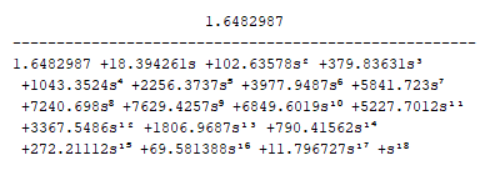
\includegraphics{h_analog_lowpass.png}
    \caption{Screenshot from SCILAB Console.}
\end{figure}

\subsection{Analog Bandpass Transfer Function}
This can be obtained by replacing s$_\text{L}$ with F(s), the frequency transformation that we had employed earlier:
\[s_L \leftarrow F(s) = \frac{s^2 + \Omega_0^2}{Bs}\]
\textbf{H$_{\text{analog, BPF}}\text{(s)}$}
\begin{figure}[h]
    \centering
    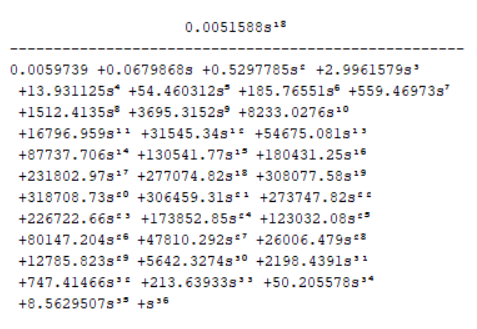
\includegraphics{h_analog_bandpass.png}
    \caption{Screenshot from SCILAB Console.}
\end{figure}

\subsection{Discrete Time Bandpass Transfer Function}
This can be obtained by applying the bilinear transformation to s:
\[s \leftarrow \frac{1 - z^{-1}}{1 + z^{-1}}\]
\textbf{H$_{\text{discrete time, BPF}}\text{(z)}$}
\begin{figure}[h]
    \centering
    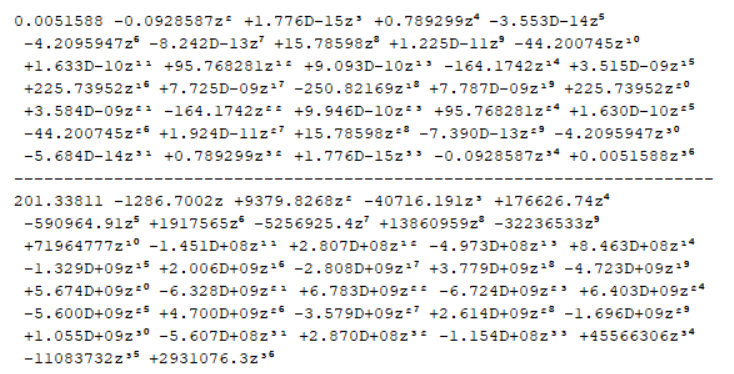
\includegraphics[width=\textwidth]{h_discrete_time_bandpass.png}
    \caption{Screenshot from SCILAB Console.}
\end{figure}

\section{Review}
I have reviewed Abhijeet's report and certify it to be correct.

\section{Plots}
Here are some plots generated using SCILAB:
\newpage
\begin{figure}[!h]
    \centering
    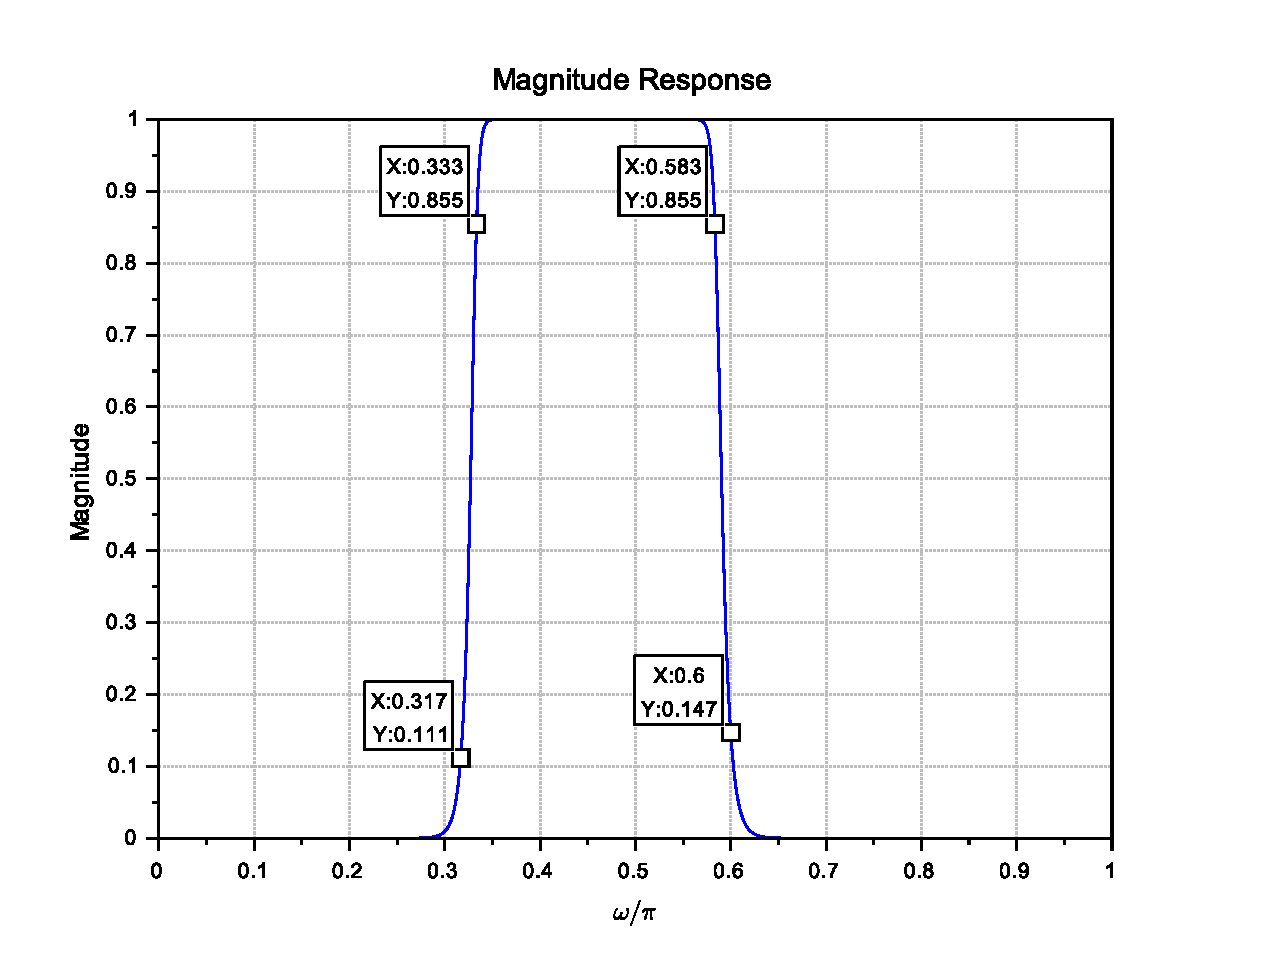
\includegraphics[scale=0.6]{mag.pdf}
% \end{figure}
% \begin{figure}[!h]
%     \centering
    \quad
    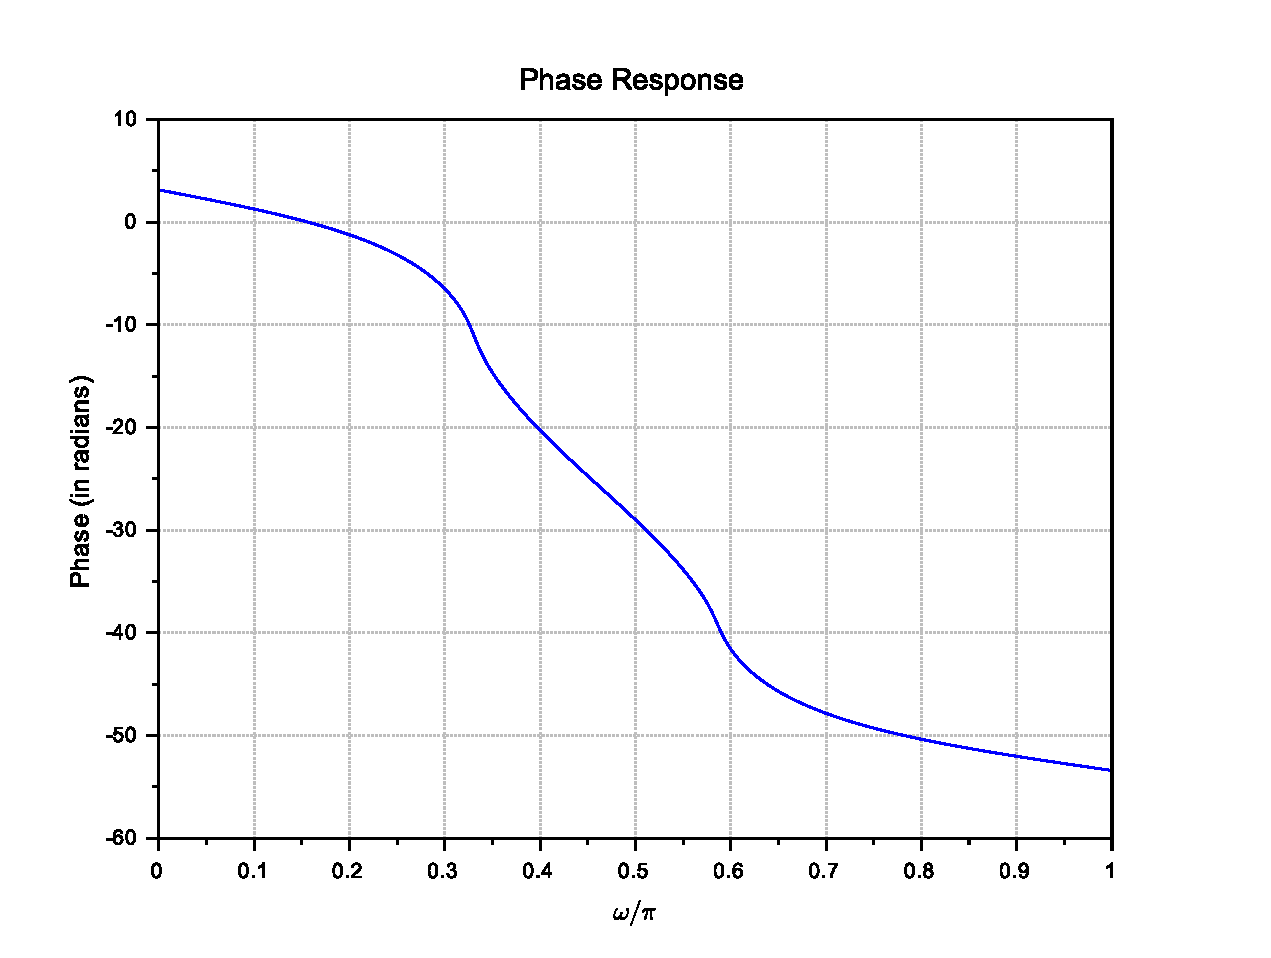
\includegraphics[scale=0.6]{phase.pdf}
\end{figure}
\begin{figure}[!h]
    \centering
    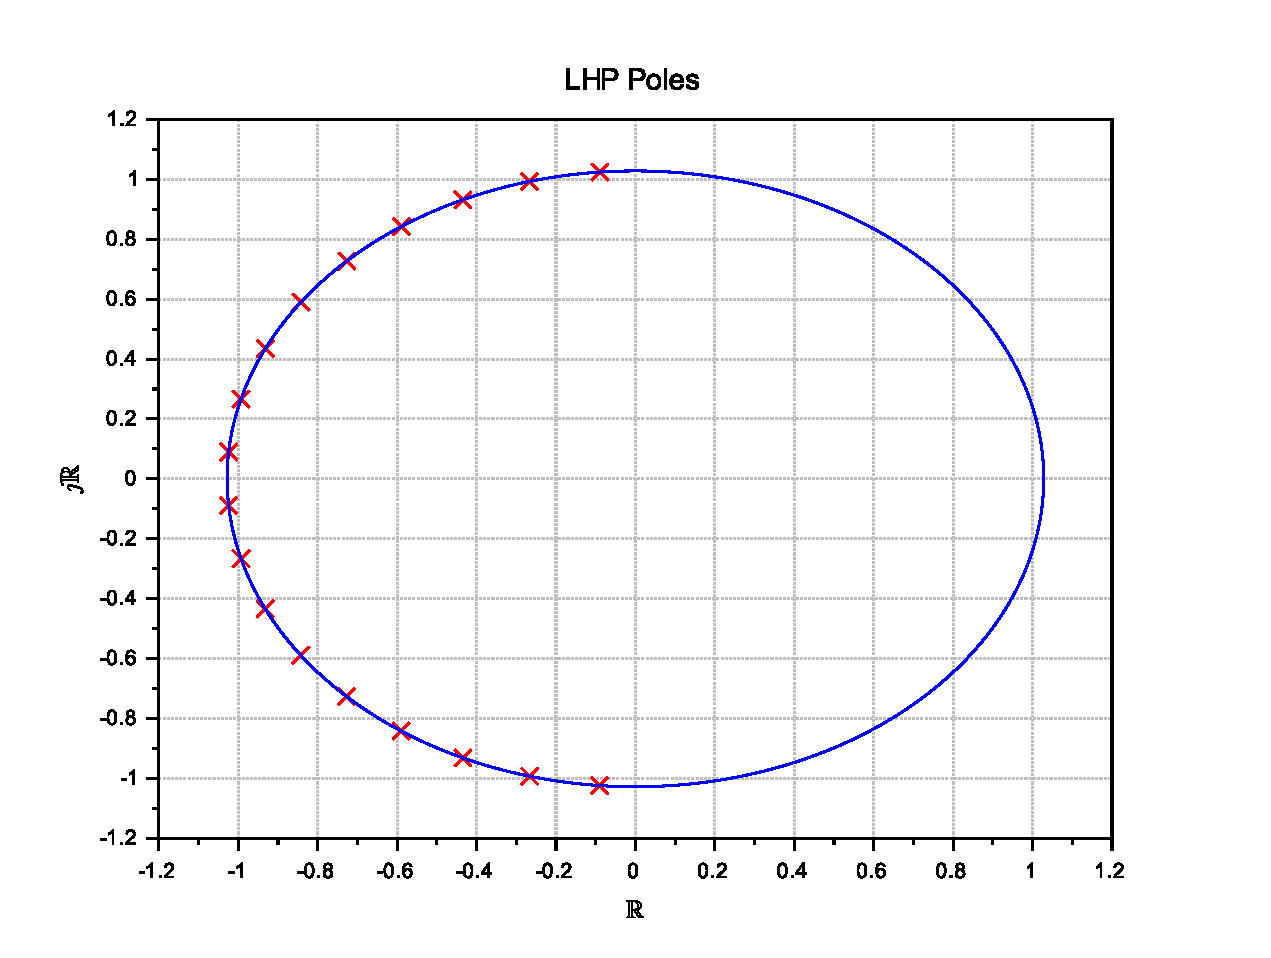
\includegraphics[scale=0.6]{poles.pdf}
    \caption{Poles of the Butterworth lowpass transfer function.}
\end{figure}

\end{document}
